% 12 variables in here:
% u_1 = 0.0, h_1 = 10.0, U_1 = 0.0, H_1 = 10.0, u_2 = 0.0, h_2 = 10.0, U_2 = 0.0, H_2 = 10.0, u_3 = 0.0, h_3 = 10.0, U_3 = 0.0, H_3 = 10.0
\begin{figure}[h!t]
\centering
  \subfigure[Height and impulse of $p_1^L$, $p_1^R$, $p_3^L$ resp. $p_3^R$.] {
    %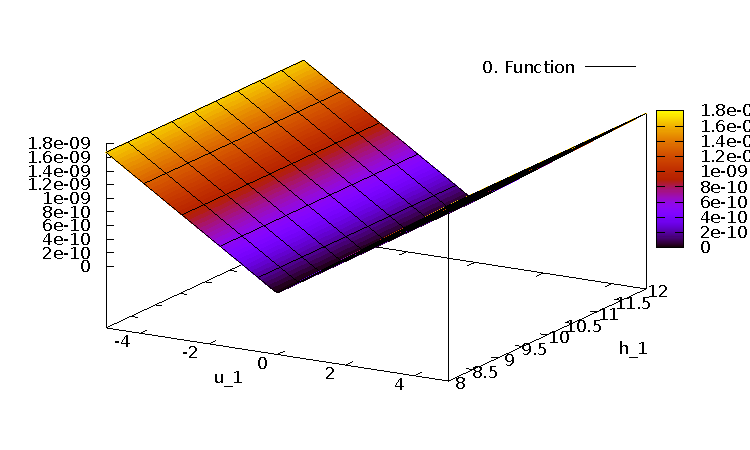
\includegraphics[scale=\zoomfactor]{{{3_punkte_equidist_alles_gleich/x_y_0.0_10.0_0.0_10.0_0.0_10.0_0.0_10.0_0.0_10.0f0}}}  
    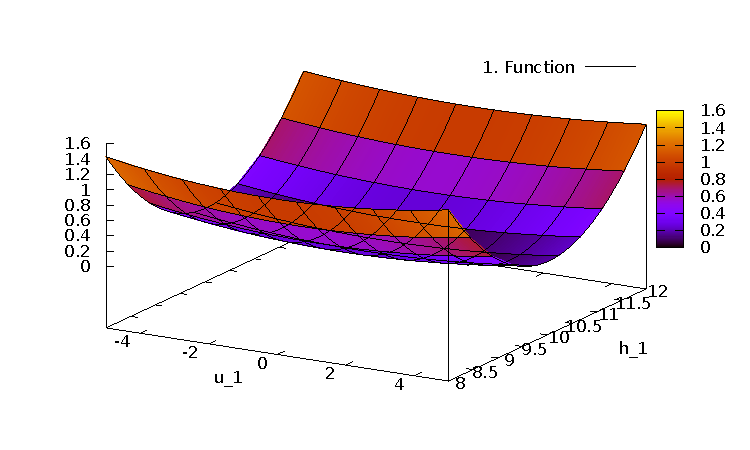
\includegraphics[scale=\zoomfactor]{{{3_punkte_equidist_alles_gleich/x_y_0.0_10.0_0.0_10.0_0.0_10.0_0.0_10.0_0.0_10.0f1}}}  
  }
  \subfigure[Height and impulse of $p_2^L$ resp. $p_2^R$.] {
    %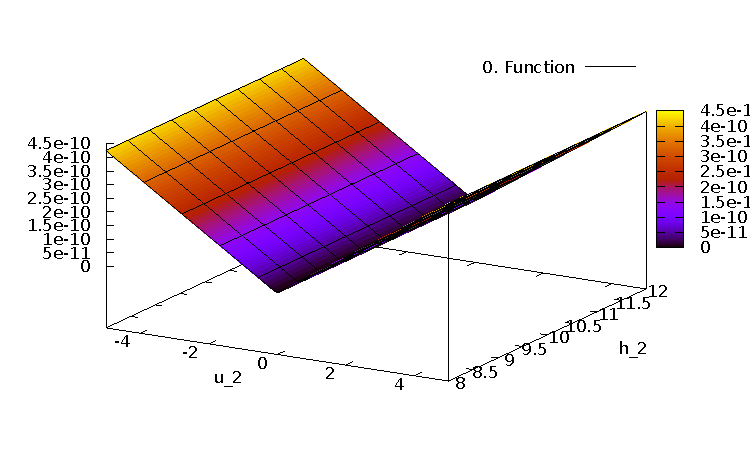
\includegraphics[scale=\zoomfactor]{{{3_punkte_equidist_alles_gleich/0.0_10.0_0.0_10.0_x_y_0.0_10.0_0.0_10.0_0.0_10.0f0}}}  
    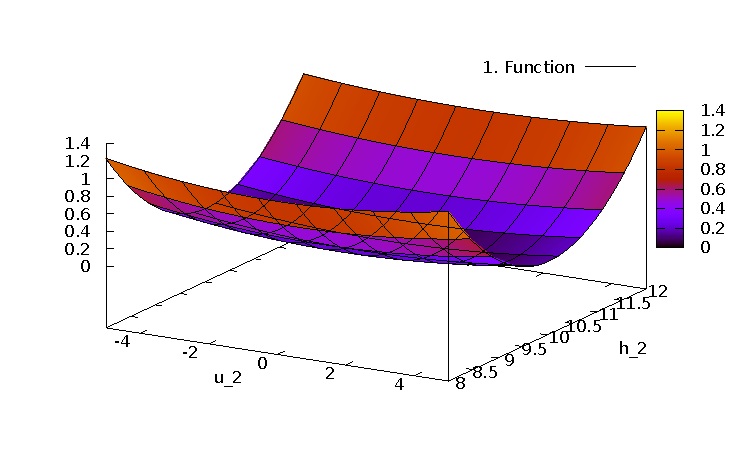
\includegraphics[scale=\zoomfactor]{{{3_punkte_equidist_alles_gleich/0.0_10.0_0.0_10.0_x_y_0.0_10.0_0.0_10.0_0.0_10.0f1}}}  
  }
  % \subfigure[Height and impulse of $p_3^L$ resp. $p_3^R$.] {
  %   %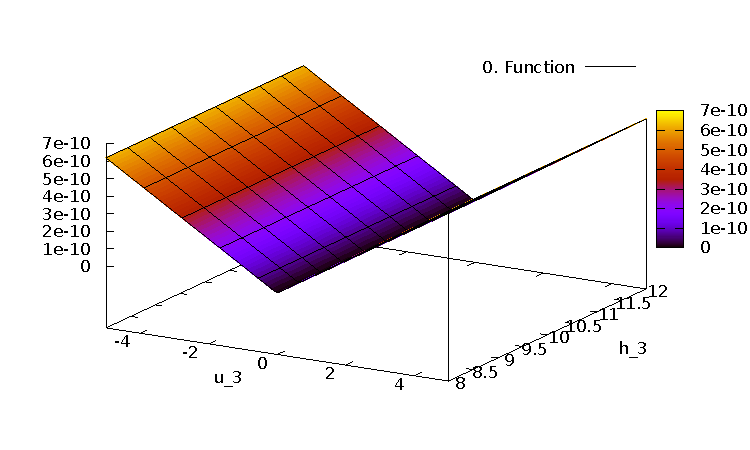
\includegraphics[scale=\zoomfactor]{{{3_punkte_equidist_alles_gleich/0.0_10.0_0.0_10.0_0.0_10.0_0.0_10.0_x_y_0.0_10.0f0}}}  
  %   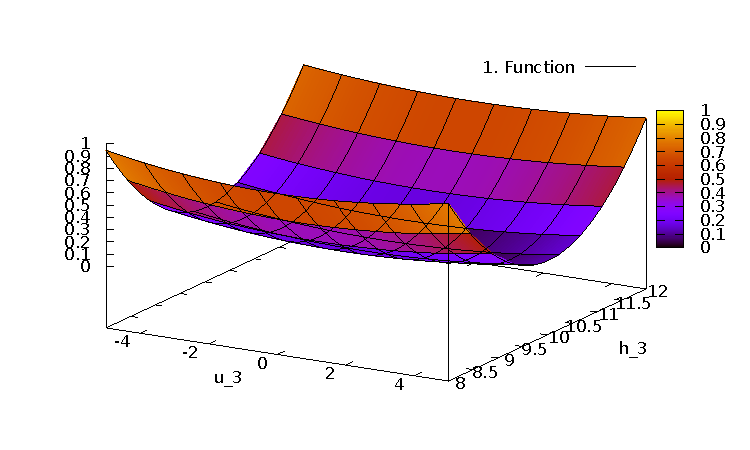
\includegraphics[scale=\zoomfactor]{{{3_punkte_equidist_alles_gleich/0.0_10.0_0.0_10.0_0.0_10.0_0.0_10.0_x_y_0.0_10.0f1}}}  
  % }
  % \subfigure[Height and impulse of $p_1^R$.] {
  %   %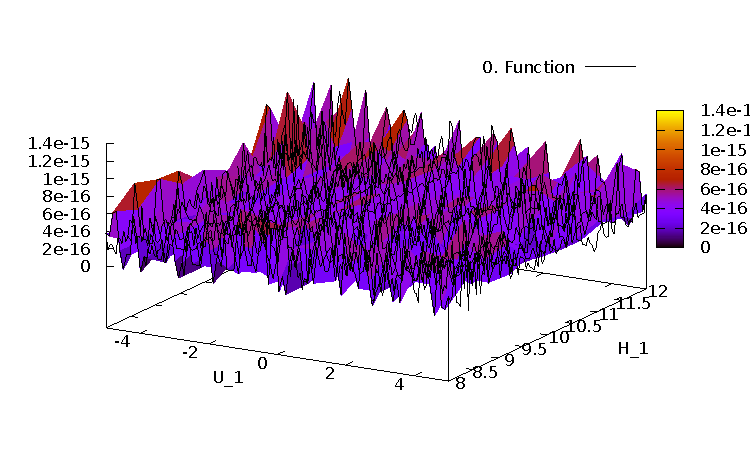
\includegraphics[scale=\zoomfactor]{{{3_punkte_equidist_alles_gleich/0.0_10.0_x_y_0.0_10.0_0.0_10.0_0.0_10.0_0.0_10.0f0}}}  
  %   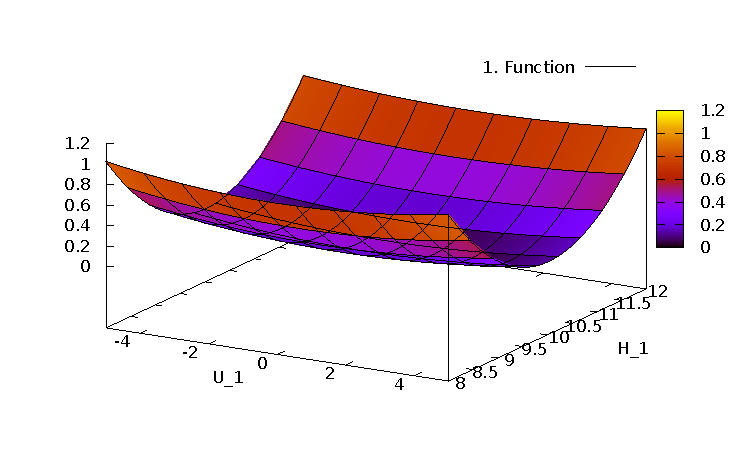
\includegraphics[scale=\zoomfactor]{{{3_punkte_equidist_alles_gleich/0.0_10.0_x_y_0.0_10.0_0.0_10.0_0.0_10.0_0.0_10.0f1}}}  
  % }
  % \subfigure[Height and impulse of $p_2^R$.] {
  %   %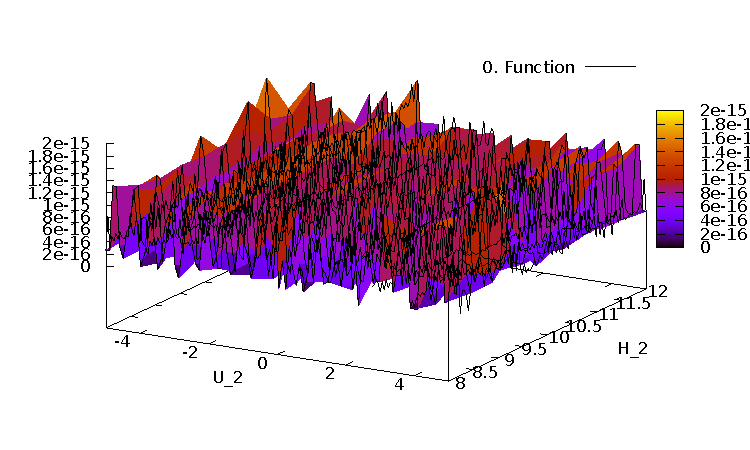
\includegraphics[scale=\zoomfactor]{{{3_punkte_equidist_alles_gleich/0.0_10.0_0.0_10.0_0.0_10.0_x_y_0.0_10.0_0.0_10.0f0}}}  
  %   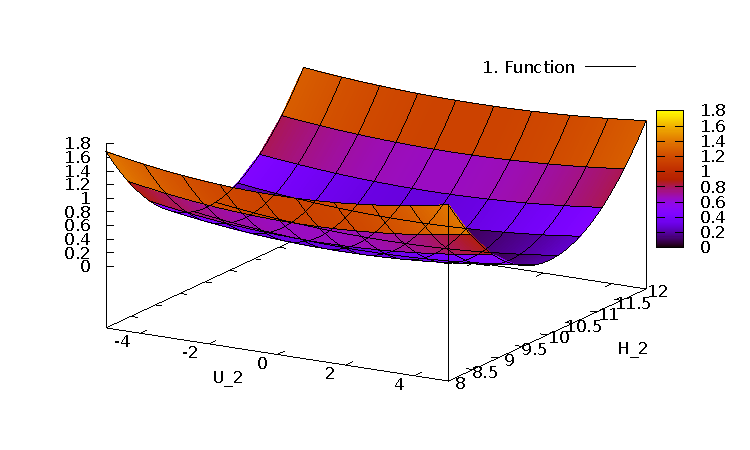
\includegraphics[scale=\zoomfactor]{{{3_punkte_equidist_alles_gleich/0.0_10.0_0.0_10.0_0.0_10.0_x_y_0.0_10.0_0.0_10.0f1}}}  
  % }
  % \subfigure[Height and impulse of $p_3^R$.] {
  %   %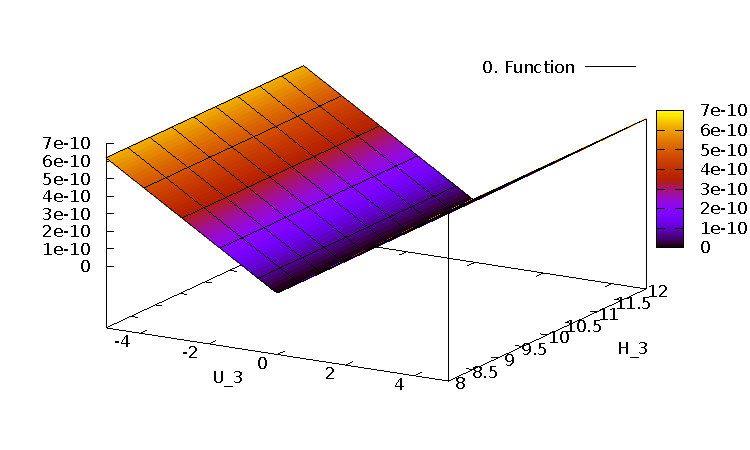
\includegraphics[scale=\zoomfactor]{{{3_punkte_equidist_alles_gleich/0.0_10.0_0.0_10.0_0.0_10.0_0.0_10.0_0.0_10.0_x_yf0}}}  
  %   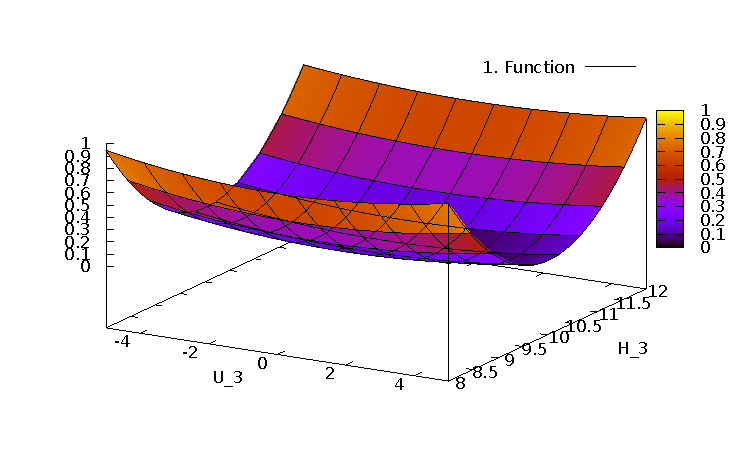
\includegraphics[scale=\zoomfactor]{{{3_punkte_equidist_alles_gleich/0.0_10.0_0.0_10.0_0.0_10.0_0.0_10.0_0.0_10.0_x_yf1}}}  
  % }
\caption{Three equidistant points. Coordinates of points are (10,0). Errors in height component are ommited since they are tiny (roughly $10^{-15}$) for each point.}
\label{fig:three-equidistant-all-fixed}
\end{figure}

%%% Local Variables:
%%% TeX-master: "../results.tex"
%%% End: